
\documentclass{article}

\usepackage{graphicx}

% title ECTQG: benchmarking road network growth models
\title{Complementarity of generative models for road networks}
\author{J. Raimbault$^{1,2,3,\ast}$\\
$^{1}$ Center for Advanced Spatial Analysis, University College London\\
$^{2}$ UPS CNRS 3611 ISC-PIF\\
$^{3}$ UMR CNRS 8504 G{\'e}ographie-cit{\'e}s\medskip\\
$\ast$ \texttt{juste.raimbault@polytechnique.edu}
}
\date{}


\begin{document}

\maketitle


\begin{abstract}
		
\end{abstract}




\section{Introduction}


Territorial systems are complex in the sense that they span across multiple dimensions, and are produced by various agents at different spatial and temporal scales \cite{batty2007complexity}. They are furthermore adaptive and self-organised, as witnesses the resilience of co-evolving city systems on long time scales \cite{pumain2021co}. Among the built environment, environmental, and social components, one crucial driver of spatial structure and dynamics of these territorial systems are transportation infrastructure networks, and more particularly road networks. They irrigate territories by distributing accessibility, and their topology and hierarchy often shapes spatial interactions and thus urban and land-use dynamics \cite{wegener2004land}. Strong effects of path-dependance furthermore highlights the role of these networks \cite{ribeill1985aspects}.

Although accessibility is nowadays strongly multimodal \cite{cats2021multi}, road networks have been the dominant transportation infrastructure in urban systems over long historical periods \cite{verdier2007extension}, and they still are an important aspect of both urban form at the microscopic scale and accessibility at the mesoscopic and macroscopic scales. Understanding the link between underlying processes driving the growth of road networks and their shape is an important subject, towards potential application to sustainable planning.

Generative processes for road networks are multiple: for example a combination of self-organisation and top-down planning may leave a significant signature in topological features of these networks \cite{barthelemy2013self}. In order to explain such evolution and in some cases reproduce existing networks, multiple simulation models have been introduced in the literature by different disciplines. These span across a broad spectrum, from data-driven models to parsimonious stylised models. \cite{xie2009modeling} propose a broad survey of such models, including economics, transport geography, transport planning and network science. The diversity of processes taken into account can range from economics of investment \cite{xie2011evolving}, to negotiations between planning stakeholders \cite{raimbault2021introducing}, full top-down planning \cite{szell2021growing}, self-organisation through morphogenesis \cite{tirico2018morphogenesis}, or local optimisation \cite{barthelemy2009co}, among others.

Most of these models include empirically documented processes, and have been validated against stylised facts such as hierarchical organisation of the network or the distribution of network measures, and also often compared against existing networks with reasonable success. However, to what extent these processes and models are complementary remains an open question. We propose in this paper a systematic benchmark of several road network growth models, to clarify the necessity of considering such diverse models. 




\section{Road network growth models}


% We include in the comparison (i) a random null model;(ii) a random potential breakdown model (Raimbault, 2020);(iii) a deterministic potential breakdown model (Raimbault, 2019);(iv) a cost-benefit compromise model ; (v) a biological network generation model (Raimbault, 2018); and (vi) a self- reinforcement model (Molinero and Hernando, 2020).
 
 \cite{raimbault2020unveiling}
 \cite{raimbault2019second}
 \cite{louf2013emergence}
 \cite{raimbault2018systemes}
  
 
 % and to compute corresponding values of diverse network measures (including betweenness and closeness centralities, accessibility, performance, diameter, density, average link length, average clustering coefficient).
  
  
\section{Results}
 
\subsection{Data}
  
  %  We use the GHSL dataset for functional urban areas worldwide and OpenStreetMap to extract real networks and population distributions for the 1000 largest urban areas,
  
 \subsection{Implementation} 
  
  %The models are integrated into the spatialdata scala library (Raimbault et al., 2020) and into the OpenMOLE software for model exploration and validation (Reuillon et al., 2013). 
  
  
\begin{figure}
\centering
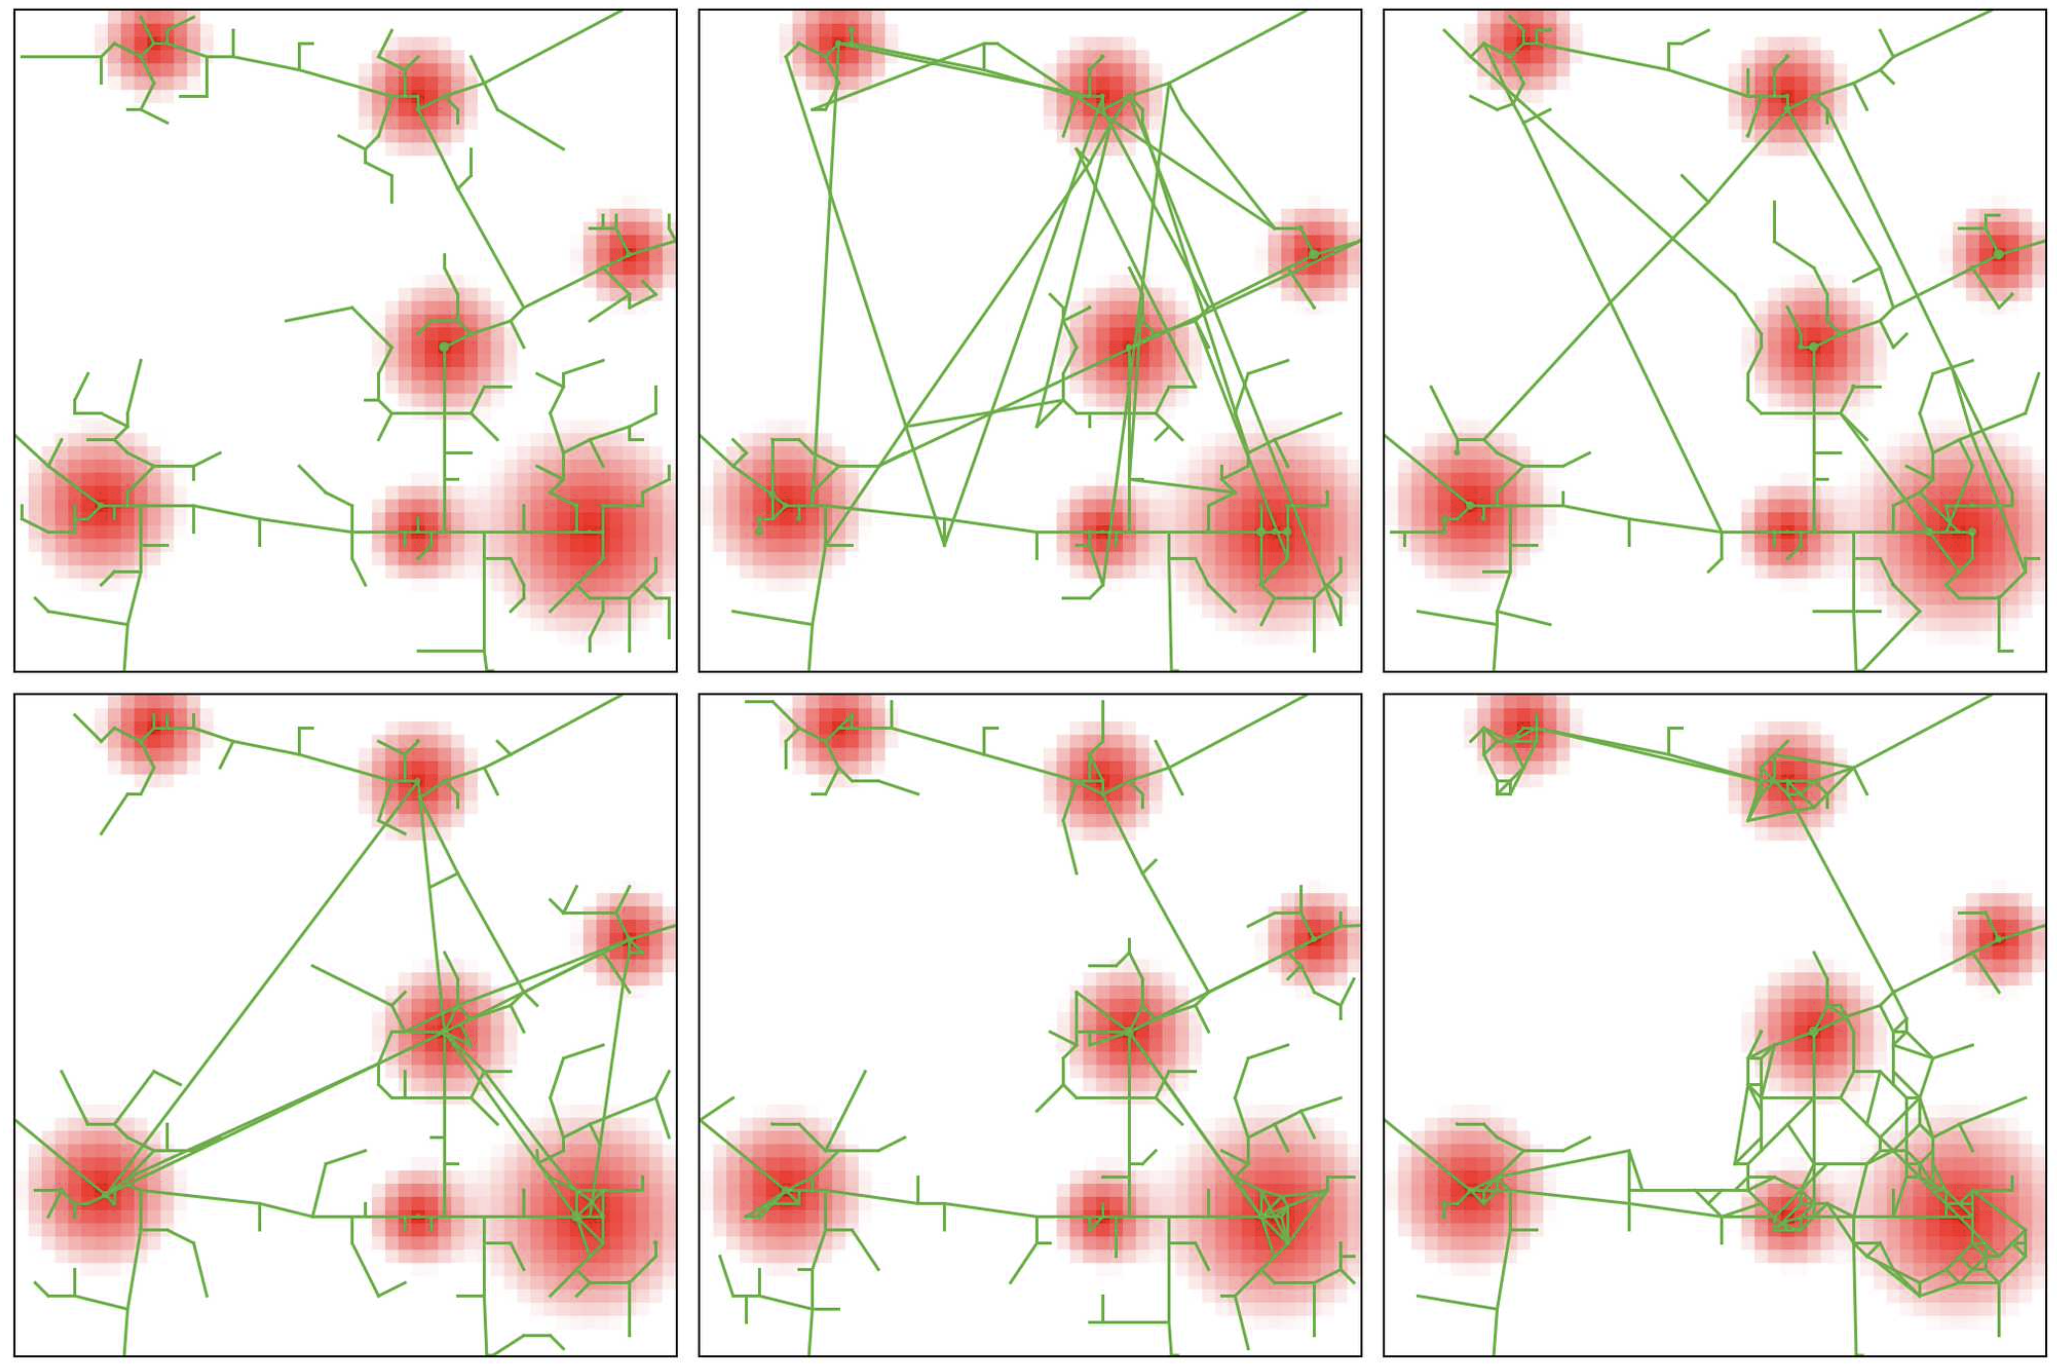
\includegraphics[width=\linewidth]{figuresraw/example-alife18.png}
\end{figure}
  
  

\subsection{Exploration}

  
%We then run a diversity search algorithm, the Pattern Space Exploration algorithm (Cherel et al., 2015), for each model with their own free parameters and with the population distribution also as input parameter among the sampled areas. This algorithm is specifically tailored to provide feasible spaces of model outputs in relatively low dimensions.
  
 %We thus proceed to a principal component analysis on real data points and project simulated values on the two first components, taken as objectives of the diversity algorithm. We obtain different shapes of feasible point clouds and corresponding effective degrees of freedom, some regions in the objective space reachable by a single model only, and a small number of urban areas which can not be approximated by the models. 


\section{Discussion}


% include more models
\cite{molinero2020model}


% This quantitatively confirms the complementarity of diverse processes driving road network growth, and the need for a plurality of models to explain it.


\bibliographystyle{apalike}
\bibliography{biblio}







\end{document}

